\chapter{Validazione non lineare nominale}
\section{Equazioni e scenari}
La campagna integra direttamente in MATLAB le equazioni SEA con i
parametri, gli attuatori e l'equilibrio descritti nei capitoli iniziali. La legge implementata è
\[
 \delta u=C_Kx_K+D_K[r;\delta q],\qquad
 \dot x_K=A_Kx_K+B_K[r;\delta q],\qquad u=\bar\tau+\delta u.
\]
Si usa \texttt{ode23t}, con tolleranze relativa $10^{-5}$ e assoluta $10^{-7}$,
passo massimo 0.005 s e uscita ogni 0.002 s. Queste prove usano MATLAB, non Simulink. Il confronto locale con la mappa
lineare è verificato automaticamente per entrambi i controllori.

Gli scenari conservano gradini di 2, 5 e 8 gradi su ciascun giunto (4 s),
disturbi lato link di 0.25, 0.5 e 1 N m (8 s), equilibrio e rumore (4 s).
L'errore statico non lineare è stimato dalla media dell'ultimo 10\% della
traiettoria. È una stima a orizzonte finito, da leggere insieme
all'assestamento; il guadagno DC lineare è una quantità distinta.

\section{Tracking, disturbi e rumore}
Gli equilibri restano invariati entro $1.7\,10^{-12}$ rad per H-infinity e
$2.3\,10^{-15}$ rad per Kmu. I gradini confermano l'assenza di overshoot
nei due controllori. Per $K_\mu$ a 5 gradi si misurano $T_s=1.522,1.484$ s,
errori relativi circa 6.03\%, 3.08\% e picchi di comando 0.796,0.199 N m.
I risultati conservano i fallimenti delle specifiche temporali di assestamento e, per Kmu sul primo
giunto, offset. Risposte e metriche di tutti i disturbi fisici sono salvate
con il controllore che le ha prodotte.

Il rumore usa esattamente due canali della sequenza encoder salvata,
con seed 20260826. La ripetizione restituisce differenza nulla.
Qui emerge un limite decisivo del candidato H-infinity: il picco di comando
è circa 5685 N m, con RMS 118.2 N m. Per Kmu si ottengono circa 8.12 N m
e 1.934 N m. Il piccolo comando nel tracking privo di rumore non descrive
dunque la sensibilità del controllore H-infinity alle misure disturbate.
Non si aggiunge una saturazione numerica per nascondere questo risultato.

\section{Regione di attrazione empirica}
La sezione iniziale conserva $\delta\theta=\delta q$, velocità nulle,
attuatori all'equilibrio e stato del controllore nullo. Restano la griglia
$\{-60,-30,0,30,60\}^2$ gradi, 36 direzioni, precisione radiale di un grado,
orizzonti 8/12 s e i criteri dichiarati nel protocollo RAS. Il superamento del limite numerico
originario $10^6$ termina anticipatamente la simulazione: quel punto avrebbe
comunque fallito il criterio di limitatezza. Le metriche di coda sono valutate
sull'uscita uniforme MATLAB. Le sezioni confrontano i due controllori robusti sullo stesso
protocollo MATLAB; non sono una RAS dei modelli Simulink originali.

Per H-infinity convergono 27 dei 285 punti esaminati; il raggio minimo risolto
è zero e il massimo circa 6.98 gradi. Zero significa che la ricerca a
risoluzione di un grado non individua un punto convergente in alcune direzioni,
non che un sistema localmente stabile abbia regione di attrazione vuota.
Per Kmu convergono tutti i 57 punti e tutti gli estremi radiali del box.
La regione è quindi limitata dal dominio esplorato, non da una frontiera
fisica identificata. Il comando massimo tra i casi convergenti raggiunge
circa 61.1 N m per H-infinity e 2763 N m per Kmu: queste regioni senza
saturazione non sono regioni operative certificate dell'hardware.
\begin{figure}[htbp]\centering
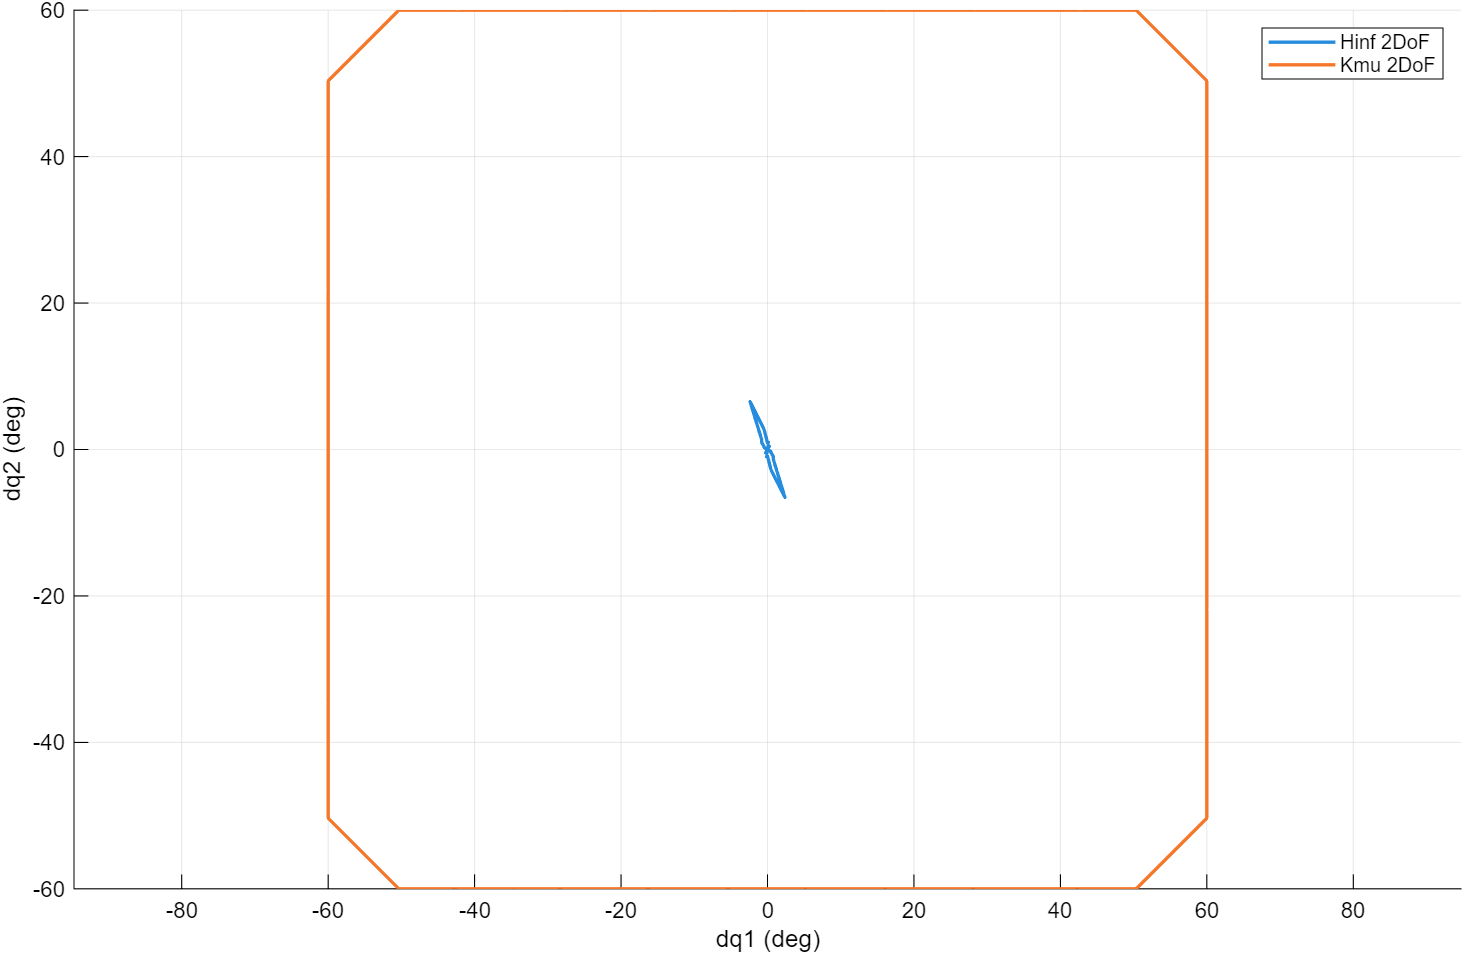
\includegraphics[width=.7\textwidth]{figures/hinf_final/ras.png}
\caption{Sezioni empiriche nominali con gli stessi criteri di convergenza.}
\end{figure}

\section{Verifica Lyapunov}
Si include l'intero stato aumentato e si risolve
$A_{cl}^TP+PA_{cl}=-I$. Per H-infinity il residuo è circa 65.27:
il controllo numerico fallisce e non si accredita alcun certificato.
Per Kmu, con 92 stati complessivi, $P$ è positiva e il residuo è 0.04493,
inferiore alla soglia preesistente 0.1. La stessa maggiorazione cubica del
resto SEA fornisce $\rho_{\mathrm{interno}}\simeq1.066\,10^{-12}$.
Il livello circa 3.697 supera la verifica su 2048 direzioni indipendenti
alle quattro frazioni radiali dichiarate; è evidenza su punti finiti,
non un'estensione del certificato analitico. Il risultato non viene trasferito a LQG o LQRI.

\section{Implementazioni MATLAB/Simulink adottate}\label{sec:originali}
Il progetto comprende otto modelli degli studenti: una coppia lineare e
non lineare per LQG, LQGI, $H_\infty$ e $\mu$-sintesi. Le copie originali
sono identificate da un manifest SHA-256. I modelli lineari usano 14 stati
fisici, quattro uscite encoder e otto ingressi nell'ordine
$[u;d;w_{link};w_u]$. Le misure rumorose alimentano il controllore,
mentre i rumori di processo sono applicati alla pianta.

LQG realizza $u=N_rr-K\hat x$ con un filtro di Kalman a 14 stati. LQGI
mantiene lo stesso osservatore e aggiunge due integratori sull'errore
misurato, $\dot\xi=r-q_{mis}$, con $u=-K_x\hat x-K_i\xi$.
Il modello $H_\infty$ confronta tre rami: il controllore 1-DoF riceve
$r-q_{mis}$, mentre 2-DoF e PID ricevono $[r;q_{mis}]$. Il modello
$\mu$ usa $K_\mu$ con la stessa interfaccia a quattro ingressi.
Le matrici dei rami 2-DoF condividono gli stati tra riferimento e misura.

I modelli non lineari integrano gli otto stati meccanici assoluti,
calcolano il disturbo sulle accelerazioni dei link e aggiungono i due
attuatori LTI. Le misure sono riportate in deviazioni dall'equilibrio
prima di essere usate dal controllore. L'inizializzazione esterna
\path{setup_student_originals.m} restituisce tutte le matrici e i tipi
Workspace necessari senza cambiare parametri o collegamenti interni.

L'ispezione ZIP/XML verifica segni, interfacce e varianze nei limiti di
un controllo statico. Tutti gli otto file sono R2026a Update 4; i tentativi
di caricamento con R2025b Update 4 falliscono per incompatibilità di
release. Nessuna simulazione o esportazione grafica nuova degli SLX è
accreditata. Per le figure e i dati Simulink sono predisposti comandi di
validazione nella release corretta; i grafici di questo capitolo sono
identificati esplicitamente come risultati MATLAB.

